\chapter{Introduction}\label{introchapter}
The auditory system is among the most ubiquitious of sensory systems as evidenced by the 
development of numerous strategies for the detection and processing of auditory stimuli
across several species. The processing of sound stimuli is fairly fast and in comparison
to light stimuli, sound has two main properties - it is omnidirectional and due to
its large wavelength, it isn't blocked by small objects. For instance we can hear objects
behind us or behind obstacles whereas the same isn't true for visual stimuli. These properties 
give the animal the obvious advantage of being able to react to approaching dangers that
aren't yet visible. In order to fully utilize the sound stimuli, it is therefore essential
that an animal is able to assess the direction or, to use the technical term, \emph{localize} a sound source.

Before we discuss the various sound localization methods observed in nature, we first
go through the fundamental steps involved in auditory perception. First, an object generates
an auditory stimulus which in general can be very complex. This stimulus then propagates
through a given medium (e.g. air, water) and excites the primary receiver(s) of the animal. In most
terrestrial vertebrates, these take the form of \emph{tympani} or eardrums - a pair of thin vibrating
membranes which are a component of the mechanical part of the auditory system.
Depending on the species, there may be an apparatus that focuses and amplifies the sound waves. In
humans for example, this function performed by the external ears or pinnae. 
The vibrations are then transmitted by means of a set of bony or cartilaginous elements and
converted into electrochemical signals that will be processed neuronally; see Sec. \ref{mechanicalprocessing}.

The neuronal processing system consists of building blocks called \emph{neurons} which are
connected to eachother through \emph{synapses}. The entire system is referred to as a 
\emph{neuronal net} which, through a form of computation, gives rise to representations of the stimuli
known as \emph{neuronal maps}. Each neuron of the map represents a specific property, e.g.
the position in space or the frequency of the stimulus and neighbouring neurons respond to
similar sensory inputs. Neuronal maps serve to reconstruct stimuli as optimally as possible
within the limits of processing. The precise calibration of the
synapses required for stimulus reconstruction is a result of experience-based learning
processes that take into account inputs from all available sensory systems.

The primary focus of this thesis is the mechanical processing that is responsible for the
sound localization ability of certain terrestrial vertebrates. Specifically, we are interested
in the analytical treatment of hearing in animals that have their eardrums connected through a large mouth cavity and the emergence of
 directionality in the response of such systems. Although our model can be scaled to several different species,
 for the purposes of a thorough comparison, we will be putting a special emphasis on lizard hearing. The questions posed by the neuronal processing of auditory stimuli in these
animals although interesting, are beyond the scope of this thesis.

\section{Mechanical Processing of Auditory Stimuli}\label{mechanicalprocessing}
Ancestors of most modern vertebrates including frogs, turtles, lizards, birds, crocodilians and mammals
developed a pair of tympani (thin vibrating membranes) to detect incoming sound waves and transmit
them from the air to the ossicles in the middle ear; cf. Fig. \ref{vertebrateearevolution}. 
Despite the large variation in size and shape, two groups with fundamentally distinct constructions can be
made out. Mammals posses tympani that are effectively separated from and therefore acoustically 
independent of each other. In contrast, the other group consisting of reptiles (lizards, turtles, crocodiles), birds and frogs
have \text{Internally Coupled Ears} (for reviews see \cite{carrsoares}, \cite{dalsgaardcarr} and \cite{schnuppcarr}) wherein
the tympani are connected through large Eustachian tubes as illustrated in \ref{lizardheadcrosssection}. The evolutionary 
appearance of independent and coupled ears (Fig. \ref{vertebrateearevolution}) suggests that the latter are probably early
tympanic ears.
\begin{figure}[ht!]
 %\centering
 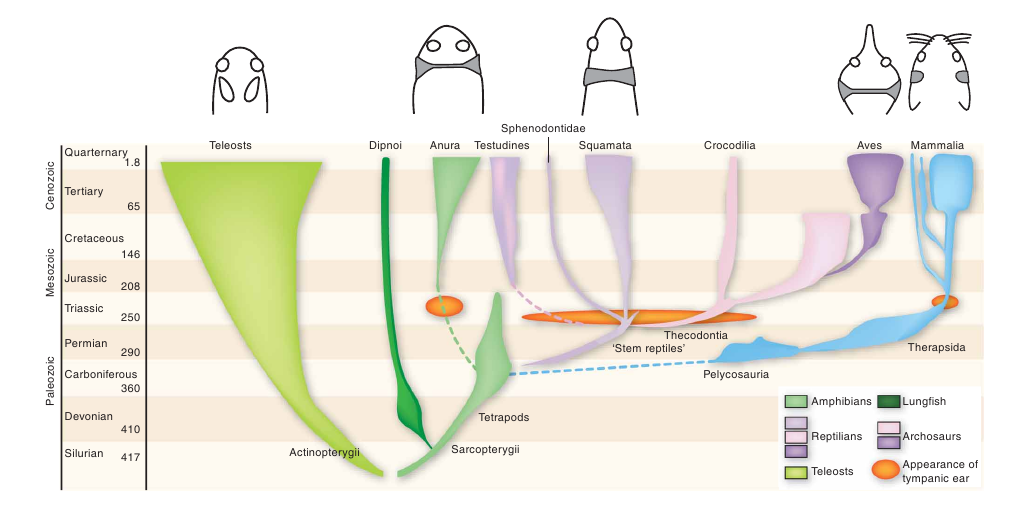
\includegraphics[width=1.0\linewidth]{Diagrams/vertebrateearevolution.png}
 \caption[Vertebrate Ear Evolution]{Evolution of vertebrate ears. Tympanic
 middle capable of receiving airborne sound evolved independently among the ancestors of modern frogs, turtles, lizards, birds,
 crocodilians and mammals. Diagrams at the top show cross-sections through different heads of these animals (middle ears - gray fill).
 Among these middle-ear systems two distinct groups can be observed - the anura (frogs and toads), squamata (lizards and snakes)
 and aves (birds) form one group with ears connected through differently shaped cavities and mammals with independent ears. Figure due to Schnupp and Carr \cite{schnuppcarr}.}
 \label{vertebrateearevolution}
\end{figure}

\begin{figure}[ht!]
 \centering
 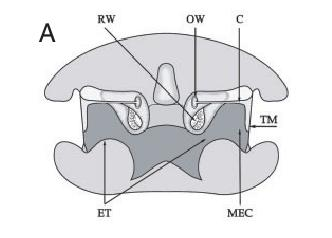
\includegraphics[width=0.4\linewidth]{Diagrams/lizardheadcrosssection.jpeg}
 \caption[Cross Section of a Lizards Head]{Diagram of the cross-section of a lizard’s head (\emph{sceloporus}). The Tympanic Membranes (TM) as well as
 the air inside the Middle Ear Cavity (MEC) and Eustachian Tubes (ET) are excited by incoming sound waves. Due to the considerable width of the Eustachian Tubes (ET), the air inside the Pharynx (P) is excited as well.
 The vibration of the tympanum causes a movement of the attached middle ear, Columella (C) whose lever construction transmits the vibrations to the Oval Window (OW), the membrane at the entrance of the fluid filled cochlea.
 Figure taken from \cite{dalsgaardmanley1}. The vibration of the OW excites the fluid in the Cochlea which gives rise to a frequency-dependent activation of the embedded basilar membrane and underlying
 auditory nerve fibers. The Round Window (RW) is a membrane at the end of the cochlea that serves to compensate the pressure within the fluid.}
 \label{lizardheadcrosssection}
\end{figure}

\section{Pressure Difference Receiving Ears}
The ability of humans and most other mammals to localize sources of sound depends on two kinds of information: the direction and frequency
of the source may cause differences between the amplitudes and arrival times of sounds reaching both ears. These pieces of information are
referred to binaural hearing cues or simply hearing cues. In mammals there is an additional source of directionality due to the shape
of the pinnae which affects the spectra of sounds reaching the ear. However, most hearing animals are lack monoaural cues and the binaural
cues are at best too small to affect the neural responses of the ears, \cite{michelsen1}. These animals are in general too small in comparison
to the wavelength of sound in their typical hearing range to cause an appreciable amplitude differences due to diffraction. Nevertheless, 
the eardrum vibration amplitude has been found to vary strongly with direction. In order to reslove this apparent paradox it was
suggested by Autrum \cite{autrumjcomphys} that the directionality could be a result of the ears vibrating due to the
differences between the pressure on the inner and outer surfaces.  The properties of such systems were also found to be analogous with the inherently directional 
nature of pressure gradient receivers studied by Harry Olson (\cite{olsonmichrophones}) was also made.


\subsubsection*{}
Our study will take place in two main steps. In Chapter \ref{modelchapter} we will
present our model for the mechanical processing of auditory signals in systems with internally coupled ears - the ICE Model.
Since our focus is on an analytical model, we would like to have a system that reduces to tractable mathematical expressions
so that we can clearly see the dependence of the system's behaviour on its parameters. To this end we will model the 
combination of the eustachian tubes, middle ear cavity and pharynx as a single continuous cylindrically shaped air cavity; see
Sec. \ref{subsecinnercavity}. The ears will be modelled as linear elastic membranes that are circular with an omitted sector
that corresponds to the extracolumella - the extension of the columella that is in contact with the ear. The
sound inputs to both the ears will be modelled as pressure waves of a given frequency with a phase difference that depends on the 
head size. The aim of the chapter is to find expressions for the quantities which give us the directional output of the system.

In Chapter \ref{modelanalysis} will evaluate the validity of our model
by comparing the calculated values of the membrane vibration velocity with experimentally determined quantities; 
see \ref{vibvelocity}. In addition to testing the directional frequency
response of the system we will also define quantities that could serve as directional cues. These two quantities are known
as the iTD (\emph{Internal Time Difference}) which measures the delay between the membrane vibrations and the iLD (\emph{Internal Level
Difference}) which measures the difference in their vibration amplitudes; Sec. \ref{hearingcuessection}. These quantities are defined in contrast to the
\emph{Interaural} Time and Level  Differences which serve as directional cues in the absence of coupling. Due to the difficulty of measurement of certain membrane
properties (e.g. fundamental frequency, damping coefficients), in Sec. \ref{parameterestimation} we will also provide means of estimating these quantities from observations.
In the final section of this chapter, Sec. \ref{vibrationpatternchapter}, we will compare the vibration profile of our model tympanum with that of a realistic tympanum and thereby
seek to explain the complex patterns of the observed.
